\chapter{Concept Generation \& Early Design}\label{ch:concept}

\begin{tipbox}[When to Read This Chapter]
\textbf{Sprint~2}: Read the full chapter. Sections on morphological charts, decision matrices, and trade studies are your primary PDR deliverables. \textbf{Sprint~3}: Return to the prototyping and BOM sections when transitioning to detailed design and procurement. \textbf{Related}: builds on Chapter~3 requirements (p.\,\pageref{ch:requirements}); feeds into PDR (Chapter~21, p.\,\pageref{ch:pdr}); prototype types connect to the integration strategy in Chapter~6 (p.\,\pageref{ch:integration}).
\end{tipbox}

\vspace{1em}

\begin{figure}[htbp]\centering
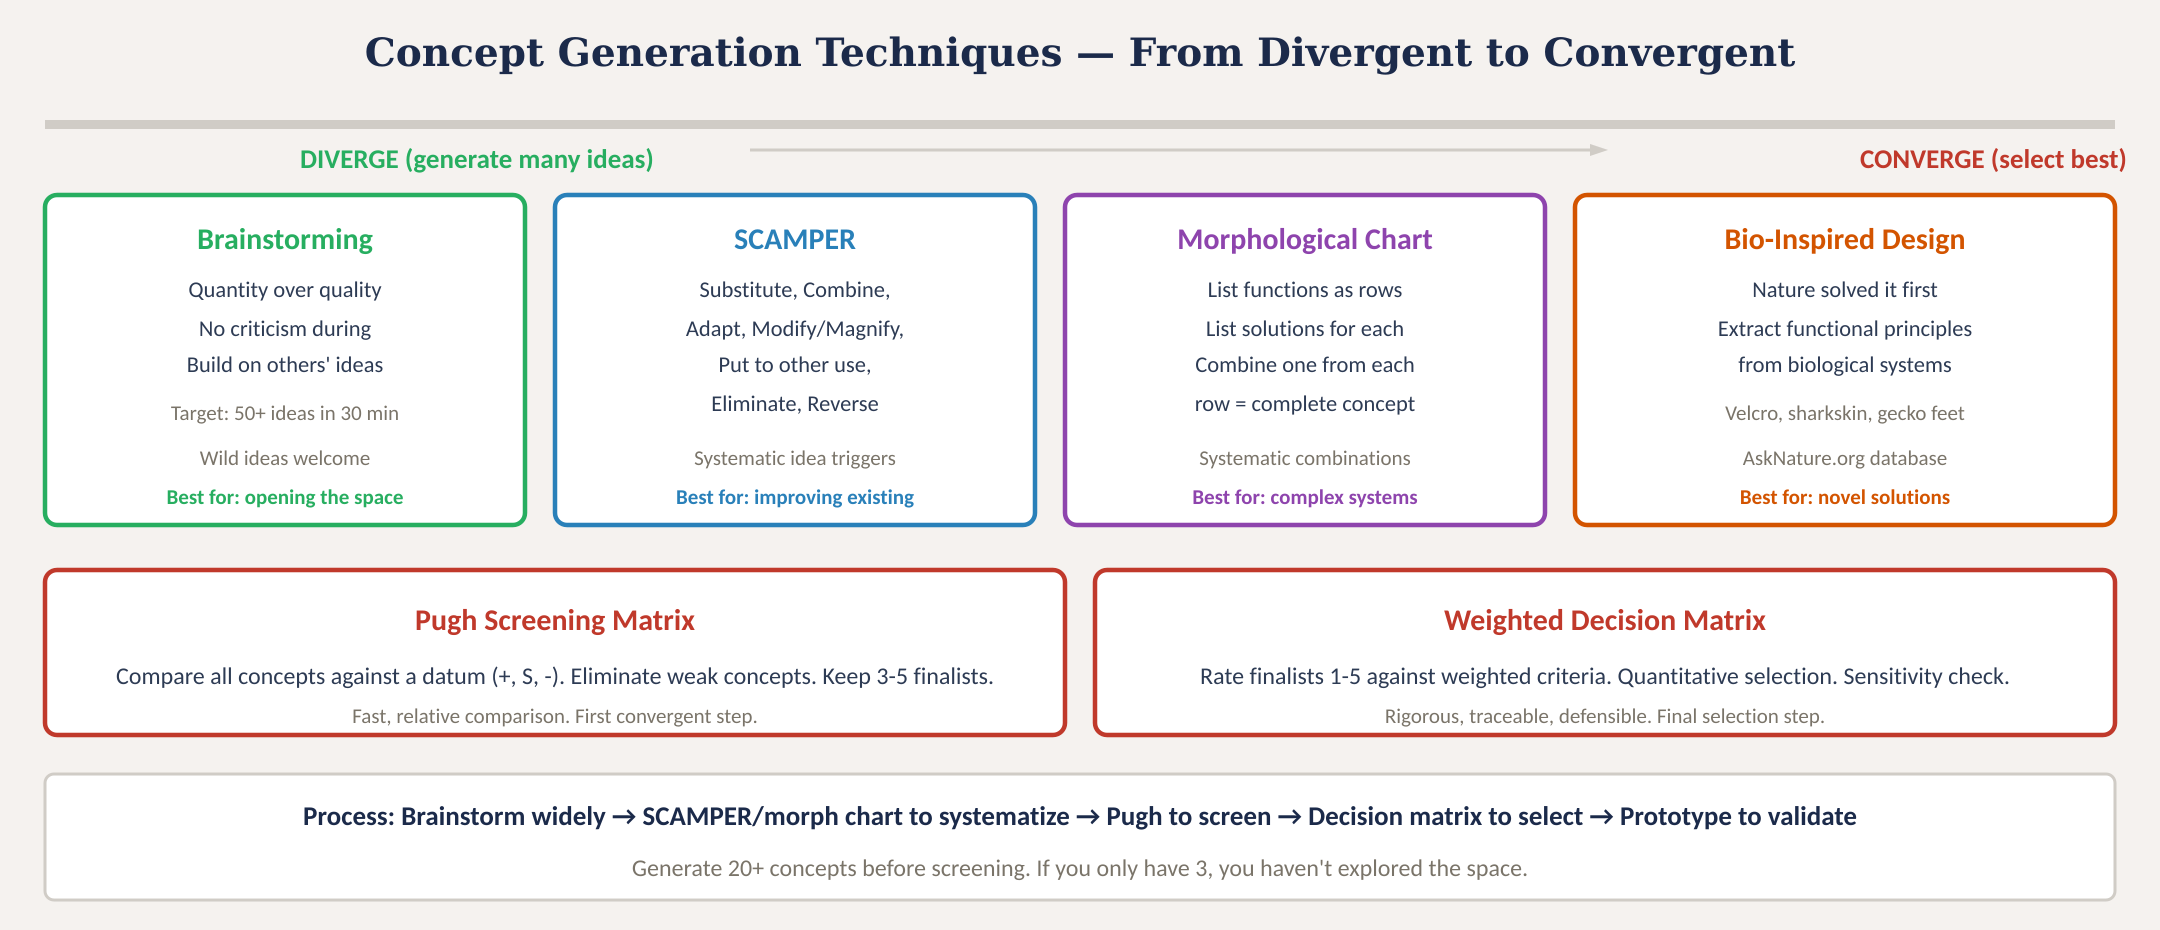
\includegraphics[width=\textwidth]{master_figs/fig_generation_techniques.png}
\caption{Concept generation techniques: divergent to convergent.}\end{figure}

\begin{figure}[htbp]\centering
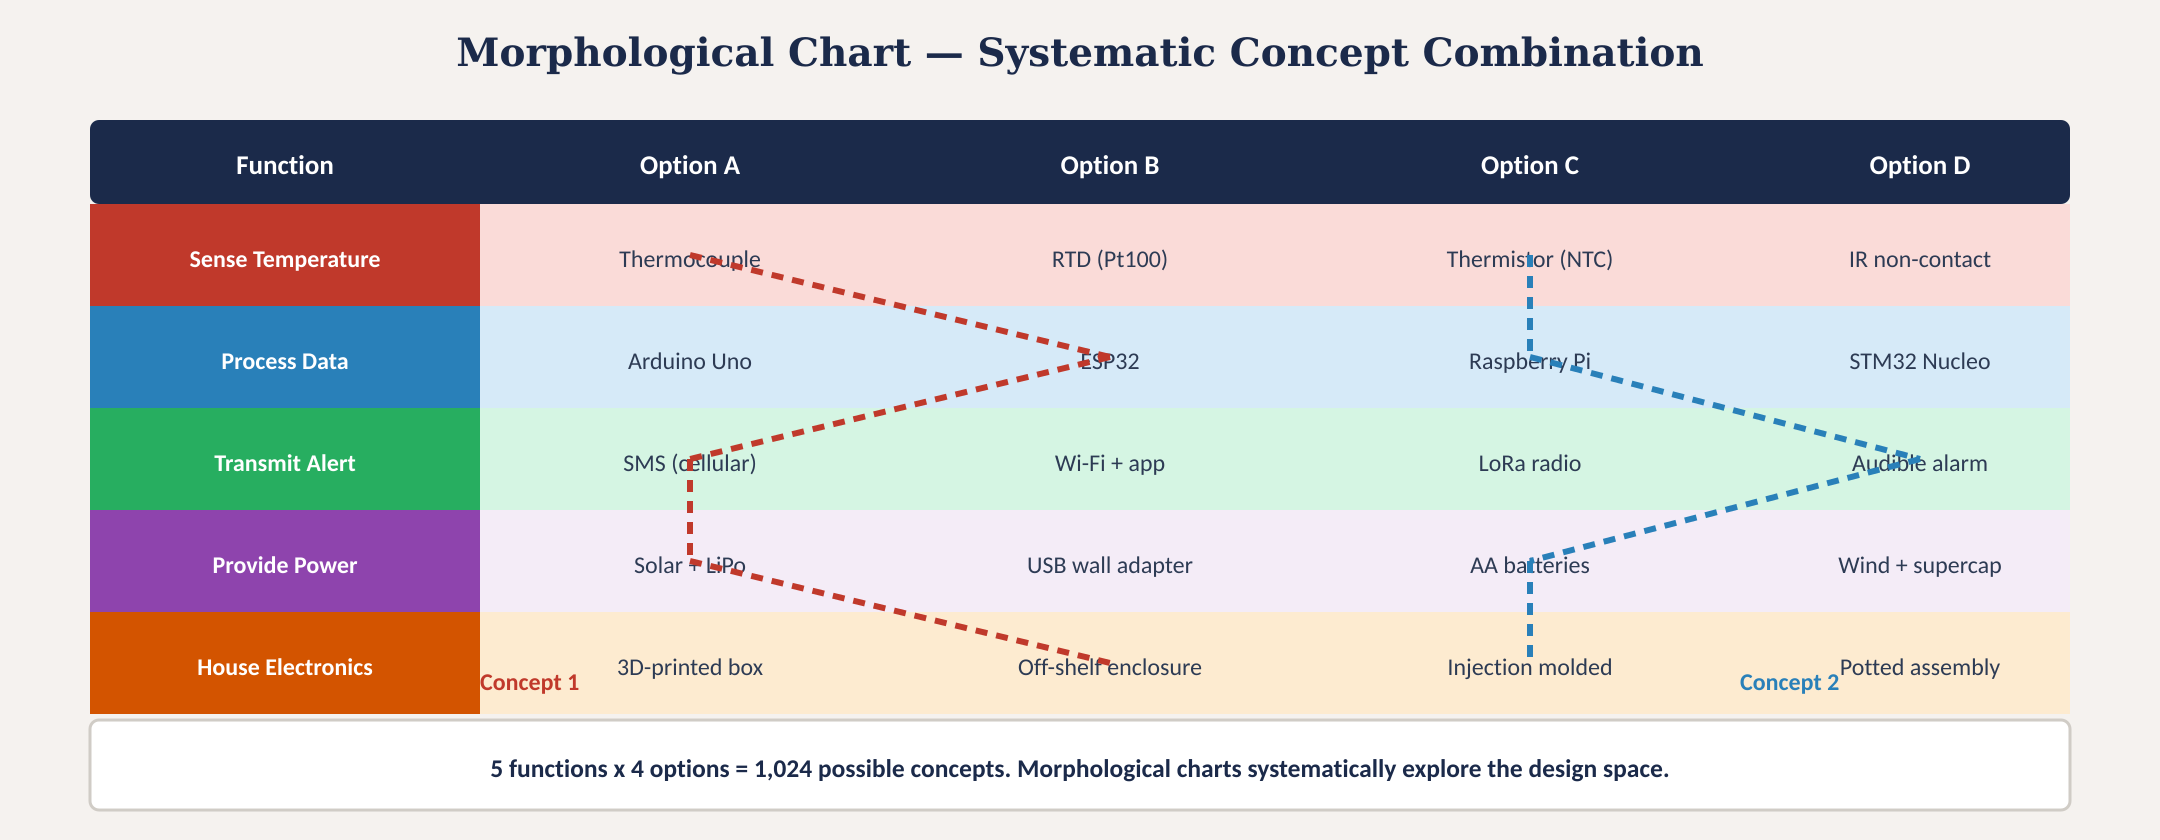
\includegraphics[width=\textwidth]{master_figs/fig_morphological_chart.png}
\caption{Morphological chart\index{morphological chart} with systematic concept combinations.}\end{figure}

\begin{figure}[htbp]\centering
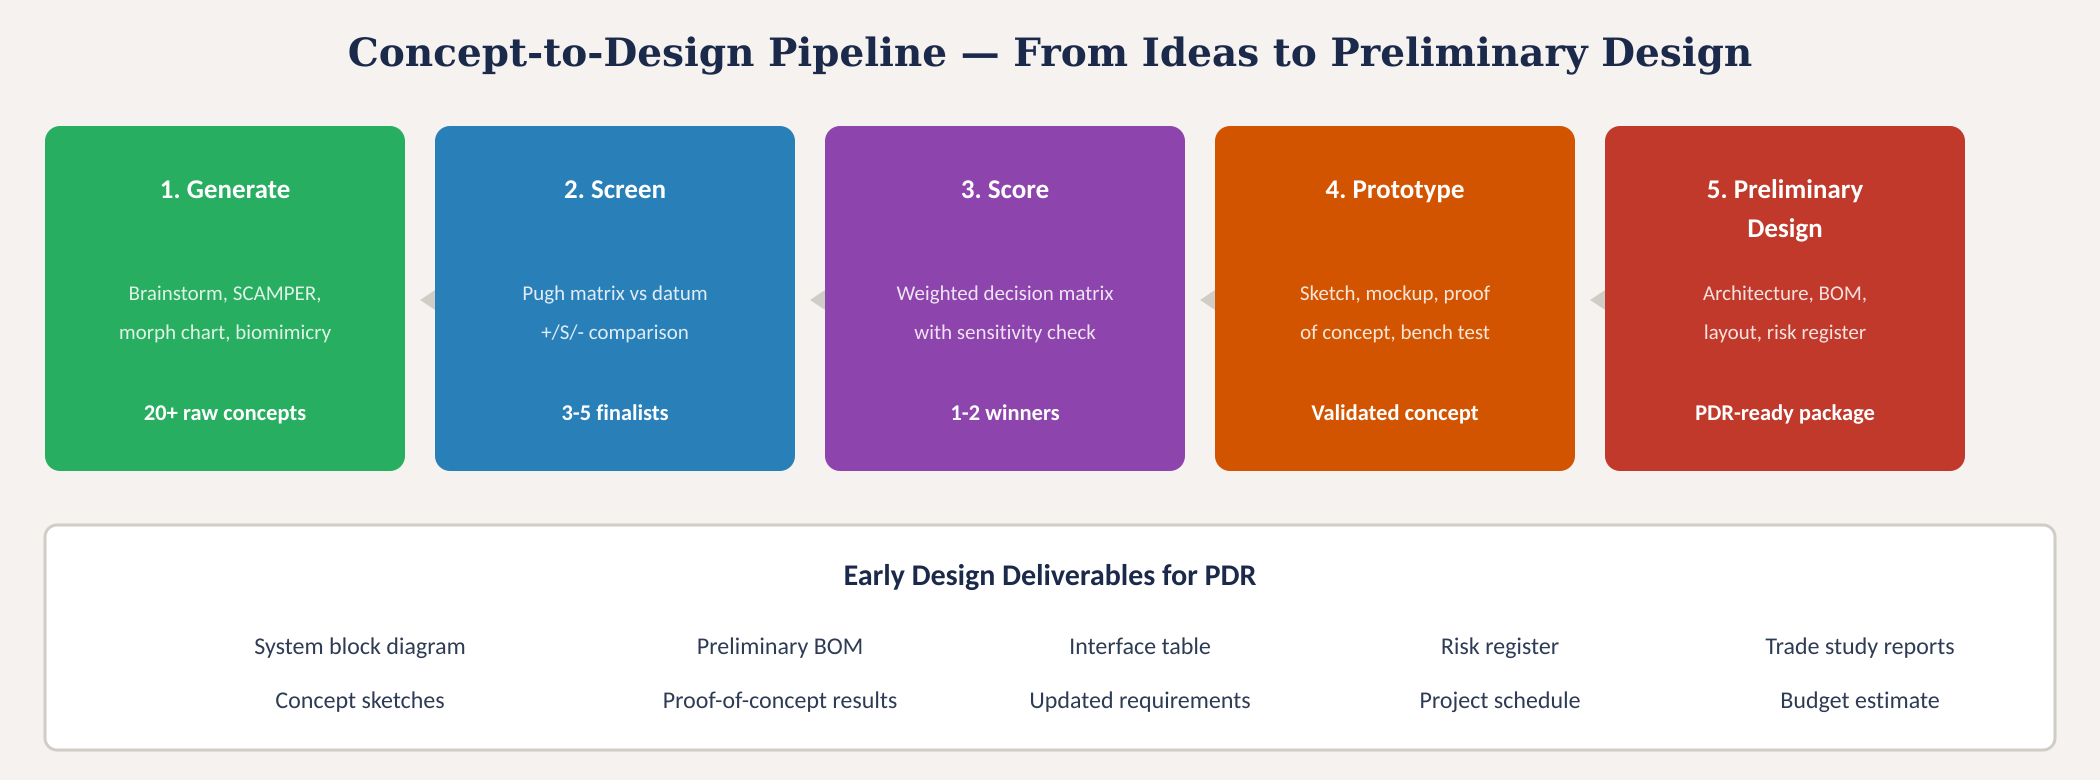
\includegraphics[width=\textwidth]{master_figs/fig_concept_pipeline.png}
\caption{Concept-to-design pipeline with PDR deliverables.}\end{figure}

\begin{figure}[htbp]\centering
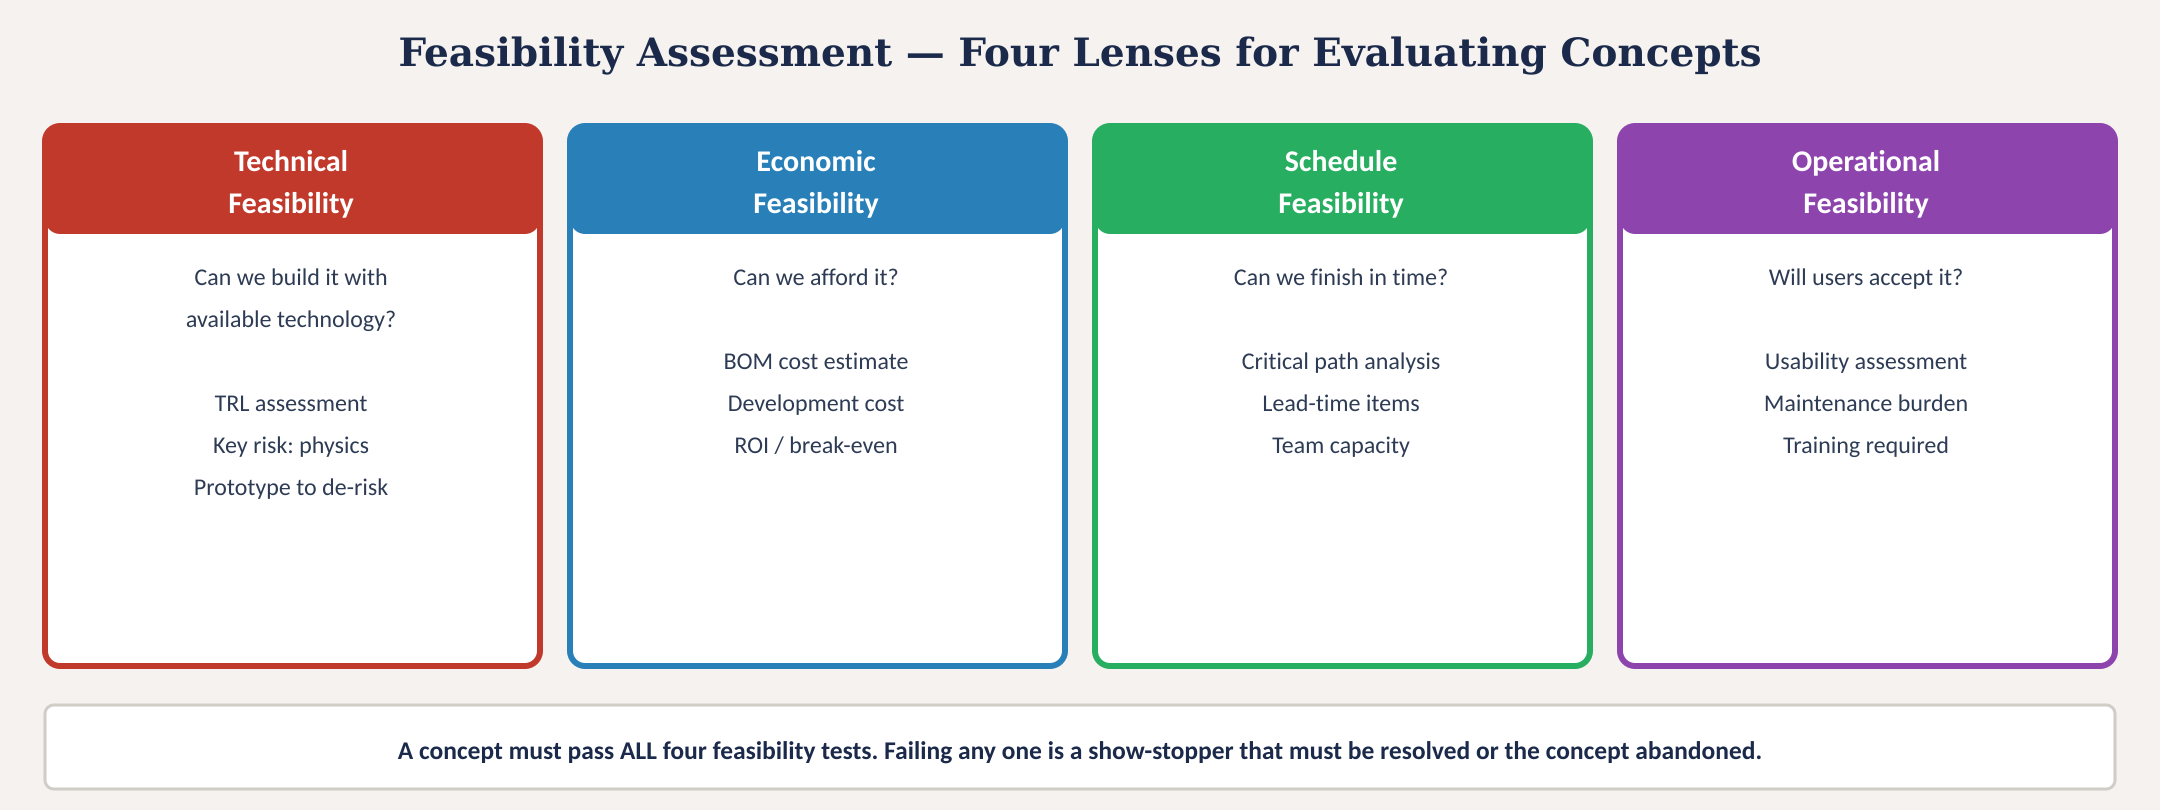
\includegraphics[width=\textwidth]{master_figs/fig_feasibility_assessment.png}
\caption{Four-lens feasibility assessment.}\end{figure}

\section{Reverse Engineering}
Reverse engineering is a structured process of disassembling an existing product to understand how it works. It builds engineering intuition and directly informs concept generation.

\subsection{The Reverse Engineering Process}
\begin{enumerate}[leftmargin=1.5em]
\item \textbf{Document the intact product}: photograph from all angles, measure overall dimensions, weigh it, record all labels and markings.
\item \textbf{Disassemble systematically}: remove fasteners in order, photograph each step, bag and label hardware. Use the right tools; forcing components causes damage that obscures design intent.
\item \textbf{Measure and catalog}: calipers for every component. Record materials (magnet test for ferrous metals, density test for plastics). Identify standard parts (bearings\index{bearing}, fasteners, seals) by markings.
\item \textbf{Create the BOM}: part number, description, quantity, material, source, estimated cost.
\item \textbf{Create an exploded view}: CAD or carefully arranged photograph with callout labels.
\item \textbf{Functional analysis}: map each component to a function. Which are structural? Functional? Cosmetic? Note any clever design solutions.
\end{enumerate}

\subsection{What Reverse Engineering Reveals}
Assembly sequence (what goes in first must come out last. DFA insight). Material choices and why they were made. Manufacturing processes (injection molding witness lines, machining marks, weld joints). Standard vs.\ custom parts ratio. Design-for-cost decisions. Failure modes on used products (wear patterns).


\subsection{Reverse Engineering Outputs}
The analysis produces artifacts that feed directly into design:
\begin{itemize}[leftmargin=1.5em]
\item \textbf{Component inventory} with identified materials and manufacturing methods; informs DFM decisions (Injection Molding chapter).
\item \textbf{Interface inventory} of all accessible mounting points, electrical connections, and mechanical features; basis for ICDs (Chapter~2).
\item \textbf{Constraint list} documenting what your design cannot change; feeds requirements as non-functional constraints.
\item \textbf{Design insights} about proven approaches, failure modes, and opportunities; informs concept generation and FMEA.
\end{itemize}

\begin{tipbox}[Non-Destructive Constraint]
In MEGN~301, you must return the COTS product undamaged at the end of each class period. No drilling, cutting, gluing, or permanent modifications. Your add-on system must interface through existing features: existing screw holes, connectors, friction fits, clamps, or custom brackets. This mirrors real-world accessory development where your product must work with an existing platform without voiding its warranty.
\end{tipbox}

\subsection{From Reverse Engineering to Concept Generation}
The reverse engineering\index{reverse engineering} analysis directly feeds concept generation:
\begin{enumerate}[nosep,leftmargin=1.5em]
\item The interface inventory defines the physical envelope and connection options for your morphological chart.
\item The constraint list eliminates infeasible concepts before time is wasted developing them.
\item Design insights from the existing product provide proven approaches to build upon.
\item The component inventory reveals standard parts that you can reuse or specify.
\end{enumerate}


\section{Generating Concepts}

\begin{figure}[htbp]\centering
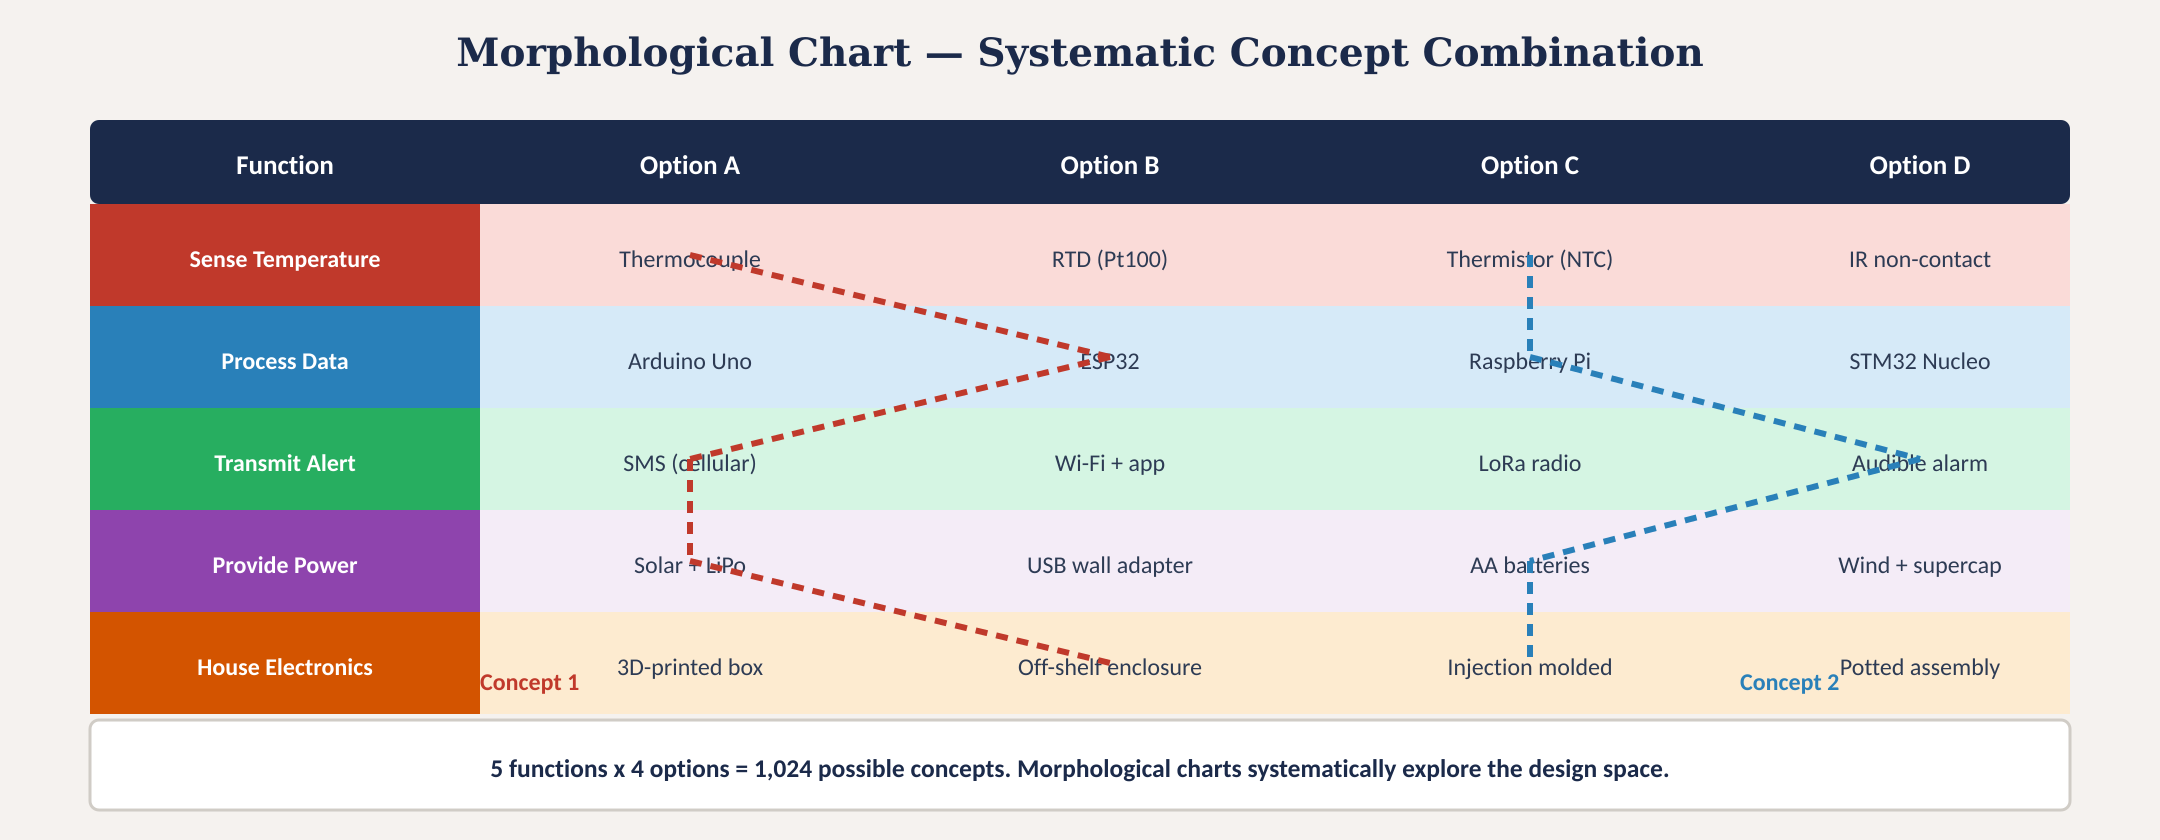
\includegraphics[width=\textwidth]{master_figs/fig_concept_process.png}
\caption{The concept generation process\index{concept generation}: from functional decomposition through systematic evaluation.}\label{fig:concept_process}\end{figure}

\subsection{Diverge Then Converge}
The concept generation process (Figure~\ref{fig:concept_process}) has two distinct phases. \textbf{Divergent} thinking generates as many ideas as possible without evaluation (brainstorming, SCAMPER, morphological charts, and bio-inspired design). \textbf{Convergent} thinking systematically evaluates and selects (Pugh screening matrices and weighted decision matrices). Generate at least 20 concepts before screening any of them.

\subsection{Brainstorming Rules}
Defer judgment (no criticism during ideation). Go for quantity (target 50+ ideas in 30 minutes). Build on others' ideas (``yes, and...''). Encourage wild ideas (they contain seeds of insight). Sketch, don't just talk.

\subsection{SCAMPER}
Seven systematic triggers: Substitute, Combine, Adapt, Modify/Magnify, Put to other use, Eliminate, Reverse. Apply each to existing concepts or competitor products to generate variations.

\subsection{Morphological Charts}
List functions as rows (from functional decomposition), brainstorm 3--5 implementation options per function as columns. A complete concept = one option from each row. A 5$\times$4 chart produces 1,024 combinations, systematically exploring the design space.

\subsection{Bio-Inspired Design}
Extract functional principles from biological systems. Velcro from burdock burrs. Sharkskin for drag reduction. Use AskNature.org to search by function. TRIZ provides 40 inventive principles for resolving design contradictions.


\subsection{Stage 1: Pugh Screening Matrix}
Rate each concept against a datum (baseline concept) as better ($+$), same ($S$), or worse ($-$). No weights, no numbers; just qualitative comparison. Sum $+$'s and $-$'s. Eliminate concepts with many $-$'s. The survivors proceed to the weighted matrix.

\textbf{Rules}: at least 3 concepts plus the datum. Criteria from requirements only. If two concepts score similarly, do not eliminate either.

\subsection{Stage 2: Weighted Decision Matrix}
Rate surviving concepts 1--5 against weighted criteria\index{sensitivity analysis} (weights sum to 1.0). Calculate weighted score per option. Check sensitivity (see Figure~\ref{fig:sensitivity} for a graphical example): vary each weight $\pm$0.05; if the winner changes, the selection is fragile.

\textbf{Common traps}: Straw-man alternatives (including clearly inferior options to make the favorite ``win''; every candidate must be legitimate). Anchoring on a favorite (assign ratings independently before group discussion). Criteria not from requirements (if a criterion does not trace to a requirement, remove it). Post-hoc weight adjustment (lock weights before scoring).

\textbf{Stage 1: Pugh Screening}: rate concepts as +/S/- against a datum. Fast, no weights. Eliminates clearly inferior options. \textbf{Stage 2: Weighted Decision Matrix}: rate finalists 1--5 against weighted criteria. Quantitative, traceable. Sensitivity check: if $\pm$0.05 weight change flips the winner, investigate further.


\section{Risk Assessment}
Risk management begins during concept selection, not after design. A \textbf{risk} is any event or condition that could prevent the system from meeting requirements. Every concept carries risks; the question is which are acceptable and which require mitigation.

\subsection{The Risk Matrix}
Risks are characterized by \textbf{likelihood} (1--5) and \textbf{consequence} (1--5). The product $L \times C$ gives the Risk Priority Number (RPN\index{RPN (Risk Priority Number)}).

\begin{table}[htbp]\centering\small
\begin{tabularx}{\textwidth}{c X X}
\toprule
\textbf{Score} & \textbf{Likelihood} & \textbf{Consequence} \\
\midrule
1 & Very unlikely ($<$5\%) & Negligible (cosmetic, workaround exists) \\
2 & Unlikely (5--20\%) & Minor (schedule slip $<$1 week, minor rework) \\
3 & Possible (20--50\%) & Moderate (schedule slip 1--2 weeks, partial redesign) \\
4 & Likely (50--80\%) & Major (missed milestone, significant redesign) \\
5 & Almost certain ($>$80\%) & Catastrophic (project failure, safety hazard) \\
\bottomrule
\end{tabularx}
\caption{Risk likelihood and consequence scales.}
\end{table}

Action thresholds: RPN 1--4 = monitor, 5--9 = mitigate, 10--15 = mitigate aggressively, 16--25 = redesign or eliminate. Maintain a risk register from PDR through FDR, updating status at each review.

\subsection{Risk Mitigation Strategies}
Four options (in order of preference): \textbf{Avoid} (change the design to eliminate the risk), \textbf{Mitigate} (reduce likelihood or consequence), \textbf{Transfer} (shift risk to a vendor, insurer, or partner), \textbf{Accept} (document and monitor; only for low-RPN items).


\begin{greenshieldbox}[GreenShield: Risk Register at PDR]
\small
\begin{tabularx}{\linewidth}{X c c c X}
\toprule
\textbf{Risk} & \textbf{L} & \textbf{C} & \textbf{RPN} & \textbf{Mitigation} \\
\midrule
Solar panel insufficient in winter & 4 & 4 & 16 & Battery margin + Dec test \\
LoRa blocked by terrain & 3 & 3 & 9 & Site survey + repeater \\
Relay fails closed (heater on) & 2 & 5 & 10 & Thermal fuse backup \\
Thermocouple accuracy inadequate & 3 & 3 & 9 & In-situ calibration \\
MCU brown-out\index{brown-out} during Wi-Fi TX & 4 & 3 & 12 & 470\,$\mu$F decoupling \\
\bottomrule
\end{tabularx}
Red-zone: solar panel (16) and MCU brown-out (12) require active mitigation before CDR.
\end{greenshieldbox}

\section{Failure Modes and Effects Analysis (FMEA)}
FMEA systematically identifies potential failure modes, their effects, and their causes \emph{during design}; before hardware exists.

\subsection{Conducting a Design-Phase FMEA}
For each component or function:
\begin{enumerate}[nosep,leftmargin=1.5em]
\item List every way it can fail (\textbf{failure modes}).
\item Determine the effect of each failure on the system (\textbf{effects}).
\item Identify root causes.
\item Rate Severity (S), Occurrence (O), and Detection (D) on 1--10 scales.
\item Calculate RPN = S $\times$ O $\times$ D. Higher RPN = higher priority for corrective action.
\item Design corrective actions for the top-5 RPN items.
\end{enumerate}

\begin{table}[htbp]\centering\small
\begin{tabularx}{\textwidth}{l l X c c c c}
\toprule
\textbf{Component} & \textbf{Failure Mode} & \textbf{Effect} & \textbf{S} & \textbf{O} & \textbf{D} & \textbf{RPN} \\
\midrule
Temp sensor & Reads high & Heater never activates; crop loss & 8 & 3 & 4 & 96 \\
Relay & Stuck closed & Heater runs continuously; fire risk & 9 & 2 & 6 & 108 \\
MCU & Brown-out reset & System offline during freeze event & 7 & 4 & 5 & 140 \\
cellular module & No signal & Alert not sent; operator unaware & 5 & 3 & 3 & 45 \\
Power supply & Fails open & Complete system loss & 8 & 2 & 7 & 112 \\
\bottomrule
\end{tabularx}
\caption{Example design-phase FMEA for GreenShield frost protection system.}
\end{table}

The MCU brown-out (RPN 140) is the highest-priority item; address it with decoupling capacitors\index{decoupling capacitor}, a voltage supervisor, and separate power routing (see Chapter~9).


\subsection{Prototype Types in Detail}
\textbf{Proof of Concept (PoC)}: validates the riskiest technical assumption. Build the minimum hardware/software to answer one question: ``Does the physics/algorithm/mechanism work?'' Example: a breadboard circuit with just the sensor and MCU to verify temperature accuracy before designing the full system. Build time: 1--3 days. Quality: ugly is fine.

\textbf{Form/Fit prototype}: verifies physical compatibility. 3D-print the enclosure, mount real components, check cable routing and assembly sequence. No electronics need to function; this is a geometry check. Build time: 2--4 days. \textbf{Always print at 1:1 scale and test-fit real components.}

\textbf{Looks-Like/Works-Like}: a near-complete system that demonstrates both form and function. This is your CDR deliverable. It should be close to the final design but may use breadboard wiring or temporary mounting. Build time: 1--3 weeks.

\textbf{Minimum Viable Product (MVP)}: the simplest version that delivers value to the stakeholder. It meets the MUST requirements but may defer SHOULD and COULD features. The MVP is what you demonstrate at FDR.

\begin{tipbox}[Build the Highest-Risk PoC First]
Identify the single technical element most likely to fail. Build a PoC for that element before anything else. If it fails, you learn early and can pivot. If it works, confidence increases and the rest of the design proceeds on solid ground.
\end{tipbox}

\begin{figure}[htbp]\centering
\begin{tikzpicture}[
    >=Stealth,
    qbox/.style={diamond, draw=MinesBlue, fill=MinesBlue!6, aspect=2.5,
        text width=2.8cm, align=center, font=\scriptsize\sffamily\bfseries,
        inner sep=1pt, line width=0.8pt},
    abox/.style={rectangle, rounded corners=3pt, draw=AccentTeal, fill=AccentTeal!10,
        text width=3.0cm, minimum height=0.9cm, align=center,
        font=\small\sffamily\bfseries, line width=0.8pt},
    arr/.style={->, line width=0.9pt, color=MinesBlue},
    lbl/.style={font=\scriptsize\sffamily, fill=white, inner sep=1pt}
]
\node[qbox] (q1) at (0,0) {Does the physics/ algorithm work?};
\node[abox] (a1) at (5.5,0) {Proof of Concept\\{\scriptsize 1--3 days, ugly is fine}};
\node[qbox] (q2) at (0,-2.5) {Does it fit the\\physical space?};
\node[abox] (a2) at (5.5,-2.5) {Form/Fit Prototype\\{\scriptsize 3D print, 1:1 scale}};
\node[qbox] (q3) at (0,-5.0) {Can the full system\\be built and demo'd?};
\node[abox] (a3) at (5.5,-5.0) {Looks-Like/Works-Like\\{\scriptsize CDR deliverable}};
\node[qbox] (q4) at (0,-7.5) {Does stakeholder\\accept the value?};
\node[abox] (a4) at (5.5,-7.5) {Minimum Viable Product\\{\scriptsize FDR deliverable}};

\draw[arr] (q1) -- node[above,lbl]{Unknown} (a1);
\draw[arr] (q1) -- node[left,lbl]{Known} (q2);
\draw[arr] (q2) -- node[above,lbl]{Unknown} (a2);
\draw[arr] (q2) -- node[left,lbl]{Known} (q3);
\draw[arr] (q3) -- node[above,lbl]{Build} (a3);
\draw[arr] (q3) -- node[left,lbl]{Done} (q4);
\draw[arr] (q4) -- node[above,lbl]{Validate} (a4);
% Return arrows from prototypes
\draw[arr,AccentTeal!60] (a1.south) -- ++(0,-0.4) -| node[below right,lbl,pos=0.25]{\scriptsize Iterate} (q2.east);
\draw[arr,AccentTeal!60] (a2.south) -- ++(0,-0.4) -| node[below right,lbl,pos=0.25]{\scriptsize Iterate} (q3.east);
\end{tikzpicture}
\caption{Prototype type decision flowchart. Start at the top: address unknowns with the simplest prototype type, iterate, and progress downward. Each stage answers a different question.}\label{fig:proto_decision}
\end{figure}

\section{Prototyping and Feasibility}

\begin{figure}[htbp]\centering
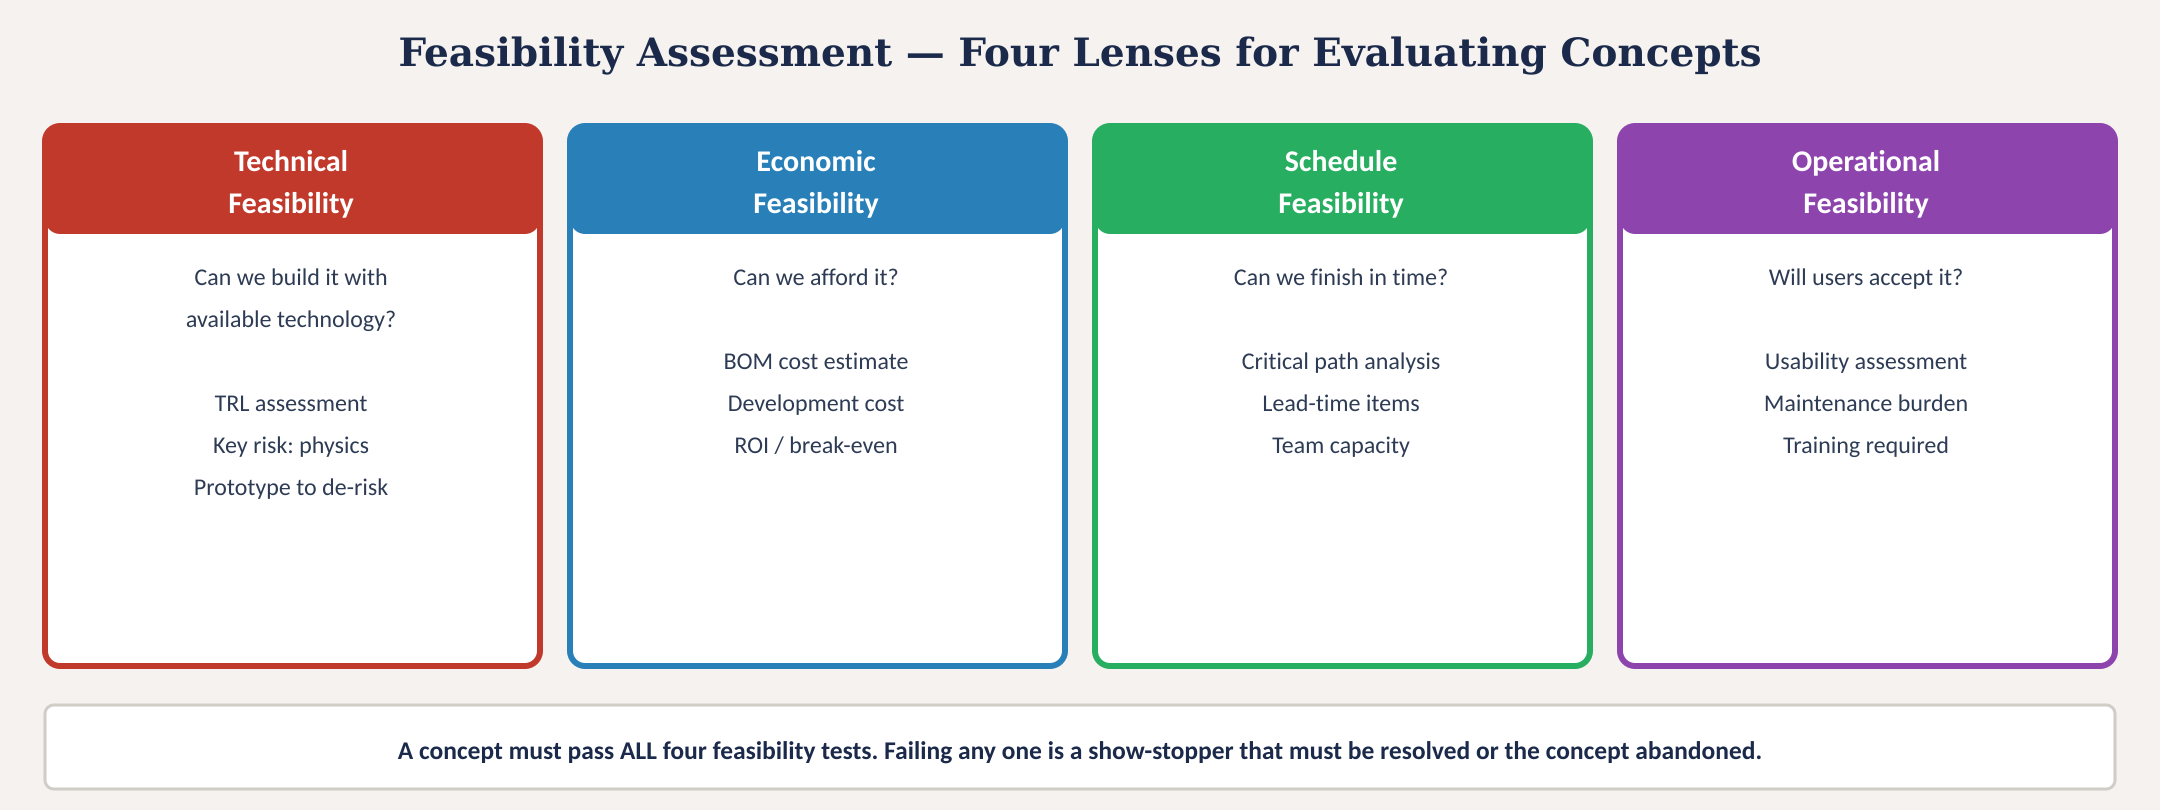
\includegraphics[width=\textwidth]{master_figs/fig_sketch_to_proto.png}
\caption{From sketch to prototype\index{prototyping}: progressive fidelity in the concept-to-hardware pipeline.}\label{fig:sketch_to_proto}\end{figure}

Four prototype types (see the progression in Figure~\ref{fig:sketch_to_proto} and the decision flowchart in Figure~\ref{fig:proto_decision}): Proof of Concept (does the physics work?), Form/Fit (does it fit the space?), Looks-Like/Works-Like (can the team build the full system?), and Minimum Viable Product (does the stakeholder accept it?). Build the PoC for the highest-risk element FIRST.

\subsection{Feasibility Assessment}
Every concept must pass four tests: \textbf{Technical} (can we build it?), \textbf{Economic} (can we afford it?), \textbf{Schedule} (can we finish in time?), \textbf{Operational} (will users accept it?). Failing any one is a show-stopper.


\section{Design Documentation}
Complete design documentation enables someone else to build, test, and maintain your system without your presence.

\subsection{Bill of Materials\index{bill of materials (BOM)} (BOM)}
Required columns: item number, part number, description, quantity, material, vendor, vendor part number, unit cost, lead time, status (ordered/received/installed). Organize hierarchically: Level~0 = system, Level~1 = subsystems, Level~2 = assemblies, Level~3 = parts. \textbf{Every part must appear in the BOM.}

\subsection{Wiring Diagrams and Schematics}
\textbf{Schematics} show electrical connections using standard symbols; the ``source code'' of hardware. \textbf{Wiring diagrams} show physical routing with connector pin assignments and wire colors/gauges. Both are required: schematics for design intent, wiring diagrams for assembly.

\subsection{Software Architecture and Flowcharts}
Document firmware with: (1) state-machine diagram showing all states and transitions, (2) data flow diagram (sensor $\to$ processing $\to$ actuator), (3) pin mapping table (GPIO $\to$ function $\to$ component), (4) communication protocol definitions (message formats, baud rates, addresses).

\subsection{CAD Models and Engineering Drawings}
CAD models define geometry. Engineering drawings communicate that geometry with dimensions, tolerances, surface finishes, and notes. Every custom part requires a drawing. Standard parts reference vendor part numbers; no drawing needed.

\begin{tipbox}[Plan B Components]
For every critical component, identify a Plan~B; an alternative from a different vendor meeting the same requirements. Lead times slip, parts go out of stock, and vendors make mistakes. A Plan~B list saves weeks of panic.
\end{tipbox}

\begin{tipbox}[Free Electronics Supplies]
Before ordering, check the MEGN~301 electronics inventory in the ME shop. Common components (resistors, capacitors, LEDs, wire, headers, breadboards) are available at no cost. Check the shared inventory spreadsheet first.
\end{tipbox}

\begin{tipbox}[The Spring Break Shipping Trap]
Orders placed the week before spring break often arrive \emph{during} break when no one is on campus. Plan so critical parts arrive at least one week before any closure. International suppliers (AliExpress, LCSC): allow 3--4 weeks. McMaster-Carr ships next-day to Golden.
\end{tipbox}

\begin{greenshieldbox}[GreenShield: Morphological Chart]
\small
\begin{tabularx}{\linewidth}{l X X X}
\toprule
\textbf{Function} & \textbf{Option A} & \textbf{Option B} & \textbf{Option C} \\
\midrule
Sense Temp & DS18B20 digital & BME280 (T/H/P) & Thermocouple + amp \\
Control Logic & ESP32 (Wi-Fi) & Arduino Nano & RPi Zero \\
Heat Actuator & Ceramic heater + relay & Heat lamp + relay & Heated water loop \\
Communication & SMS via SIM7000G & Wi-Fi + cloud & LoRa to base station \\
Power Source & 120 VAC wall adapter & 12V solar + battery & PoE \\
\bottomrule
\end{tabularx}

\textbf{Concept 1 (Grid-Connected)}: DS18B20 + ESP32 + Ceramic heater + Wi-Fi + Wall adapter. Lowest cost, simplest, requires AC power.

\textbf{Concept 2 (Off-Grid Solar)}: BME280 + ESP32 + Ceramic heater + LoRa + Solar+battery. Grid-independent, higher cost, battery sizing critical.

\textbf{Concept 3 (Industrial)}: Thermocouple + RPi + Heated water loop + SMS + PoE. Highest capability and cost.
\end{greenshieldbox}

\begin{greenshieldbox}[GreenShield: Risk Assessment for Concept 2 (Off-Grid)]
\textbf{Technical risks}: (1) Solar panel sizing for Colorado winters, December insolation is 3.5 peak sun hours vs.\ 6.5 in July. Battery must sustain 3 consecutive cloudy days. (2) LoRa range through polycarbonate glazing, 3--6\,dB attenuation at 915\,MHz.

\textbf{Schedule risk}: Solar charge controller + BMS\index{BMS (Battery Management System)} integration adds 2 weeks. If the team is behind at CDR, this is a schedule-buster.

\textbf{Economic risk}: Solar (\$25) + charge controller (\$15) + LiPo (\$20) + LoRa (\$12 ea) = \$84 for power/comms vs.\ \$8 for Concept 1.

\textbf{Verdict}: High-risk for 16-week schedule. Recommend Concept 1 with upgrade path.
\end{greenshieldbox}

\begin{keyconceptbox}[Industry SE Parallels]
\begin{itemize}[nosep,leftmargin=1.5em]
\item \textbf{INCOSE SEH 4th ed.}: Sec.\ 4.3 (Architecture Definition), Sec.\ 4.4 (Design Definition).
\item \textbf{NASA SP-2016-6105 Rev 2}: Ch.\ 4.4 (Design Solution Definition), Ch.\ 6.6 (Decision Analysis).
\item \textbf{IEEE 1220}: Standard for systems engineering process management.
\end{itemize}
\end{keyconceptbox}

\section{Artifact Handoff: What Chapter 3 Produces}
\begin{table}[htbp]\centering\small
\begin{tabularx}{\textwidth}{l X l}
\toprule
\textbf{Artifact} & \textbf{Description} & \textbf{Forward Reference} \\
\midrule
Morphological Chart & Functions $\times$ implementation options & PDR documentation \\
Trade Study / Decision Matrix & Weighted evaluation of top concepts & PDR deliverable \\
Selected Concept Package & Block diagram, preliminary BOM, risk assessment & Ch.~4, CDR \\
Design Documentation & BOM, schematics, CAD, software architecture & Ch.~5 (integration), FDR \\
\bottomrule
\end{tabularx}
\end{table}

\section{Structured Creativity Methods}
\subsection{Morphological Analysis}
Morphological analysis systematically generates concepts by combining solutions for each function:

(1) List the key functions the product must perform (sense, actuate, power, communicate, enclose).

(2) For each function, brainstorm 3--5 alternative solutions (for ``sense temperature'': thermocouple, RTD, thermistor, IR sensor, bimetallic strip).

(3) Arrange in a matrix with functions as rows and solutions as columns.

(4) Generate concepts by selecting one solution from each row and combining them. A 5-function matrix with 4 alternatives per function yields $4^5 = 1024$ theoretical combinations.

(5) Screen the combinations for compatibility (not all combinations are physically or economically feasible) and select the 5--10 most promising for detailed evaluation.

\subsection{SCAMPER Method}
A checklist for modifying existing designs: \textbf{S}ubstitute (different material, component, process), \textbf{C}ombine (merge two functions into one component), \textbf{A}dapt (borrow a solution from another domain), \textbf{M}odify (change size, shape, color, texture), \textbf{P}ut to other use (use the product for a different application), \textbf{E}liminate (remove a feature or component), \textbf{R}everse/Rearrange (change the order, orientation, or hierarchy).

\subsection{Biomimicry}
Nature has solved many engineering problems through evolution. Look to biological systems for inspiration: gecko feet for adhesion without glue, termite mounds for passive ventilation, shark skin for drag reduction, pinecones for humidity-responsive actuation, and bone structures for lightweight strength. In MEGN~301, biomimicry is particularly relevant for thermal management (how do desert animals stay cool?), fluid handling (how do trees pump water 100\,m upward?), and structural design (how do shells achieve high strength-to-weight ratios?).

\section{Concept Selection: Beyond the Pugh Matrix}

\begin{figure}[htbp]\centering
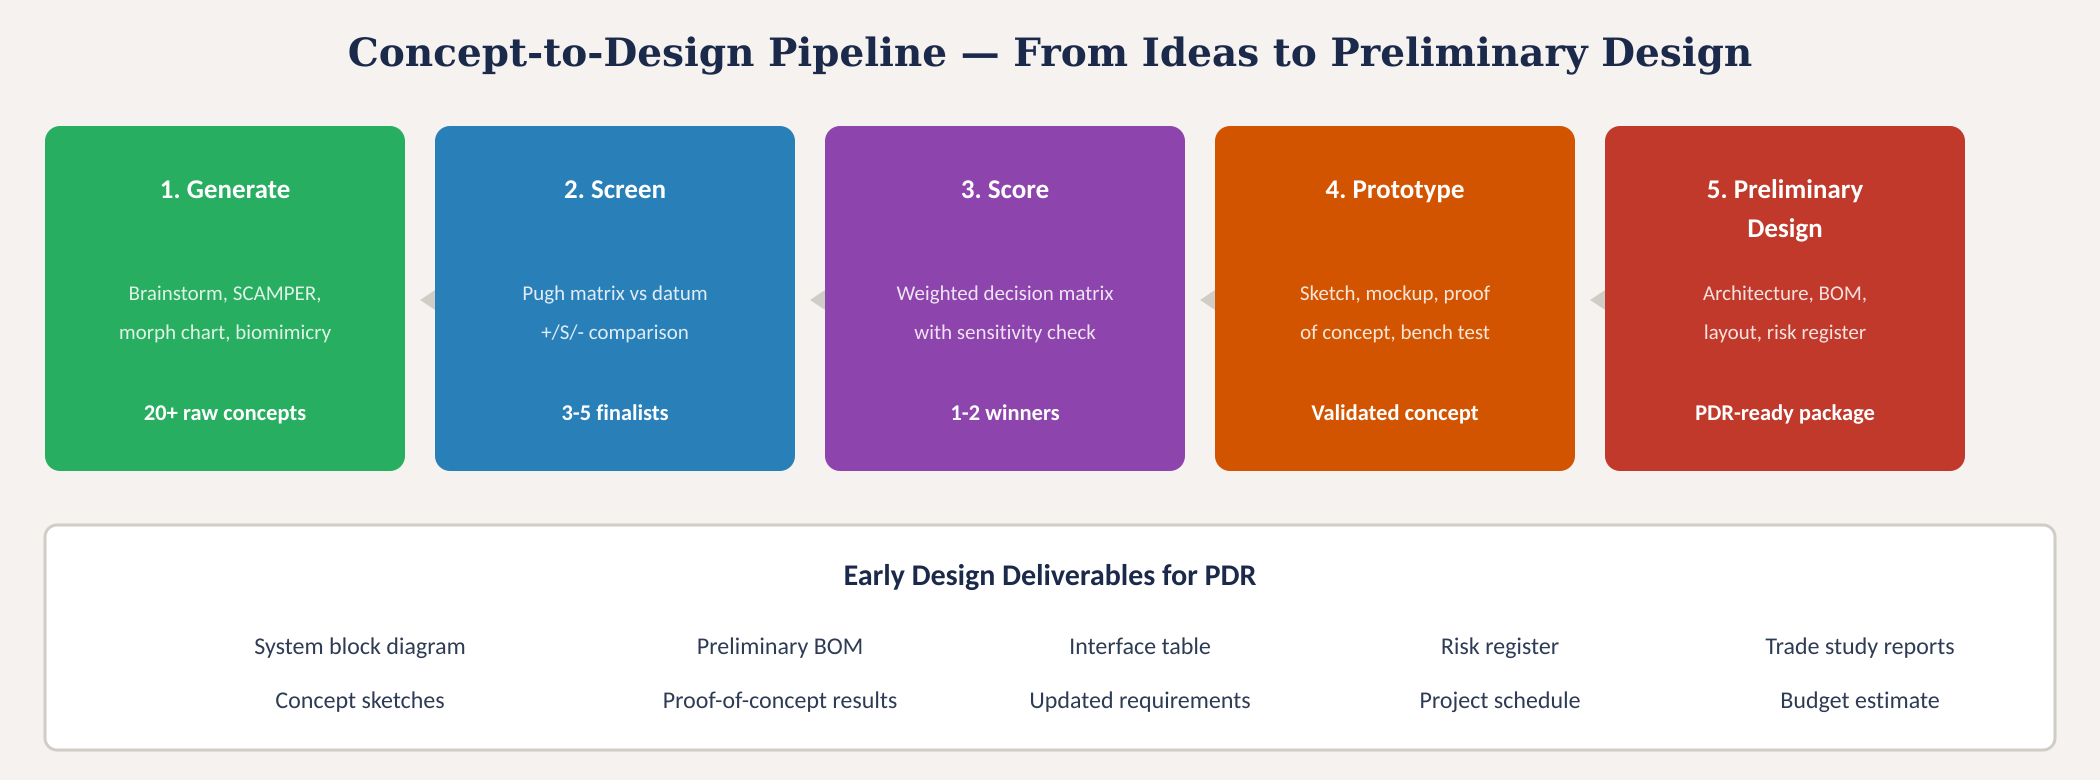
\includegraphics[width=\textwidth]{master_figs/fig_selection_funnel.png}
\caption{Concept selection funnel\index{concept selection}: from broad ideation through screening to a single committed design.}\label{fig:selection_funnel}\end{figure}

\subsection{Weighted Decision Matrix}
The concept selection funnel (Figure~\ref{fig:selection_funnel}) narrows candidates systematically. An enhanced Pugh matrix where criteria are weighted by importance:

(1) Define 6--10 evaluation criteria (performance, cost, complexity, reliability, manufacturability, safety, sustainability).

(2) Assign weights (total $= 100\%$). Typically: performance 25\%, cost 20\%, manufacturability 15\%, reliability 15\%, safety 10\%, sustainability 10\%, aesthetics 5\%.

(3) Score each concept against each criterion on a 1--5 scale.

(4) Compute weighted scores and rank.

(5) Perform sensitivity analysis: vary the weights by $\pm$20\% and check whether the ranking changes. If it does, the decision is sensitive to subjective weighting and requires careful justification.

\subsection{Concept Testing}
Before committing to a concept, build a quick proof-of-concept prototype to validate the highest-risk element. This is \emph{not} the final prototype; it is a focused experiment to answer one question: ``does this approach actually work?''

For a thermal control system: the highest risk might be ``can we maintain $\pm$1\,\degC{} with a 200\,W heater and PID control?'' Build a minimal system (heater, thermocouple, Arduino, relay) and test. The result either validates the concept (proceed) or invalidates it (pivot), saving weeks of detailed design effort.

\section{Design for the GreenShield Competition}
The GreenShield project evaluation criteria guide concept selection:

\textbf{Innovation (25\%)}: novel application of engineering principles, creative use of materials or processes, unique approach to the problem.

\textbf{Technical execution (30\%)}: quality of the requirements, design, fabrication, and testing. Meets all specified requirements.

\textbf{Sustainability (20\%)}: environmental impact assessment, design for disassembly, material selection, energy efficiency.

\textbf{Communication (15\%)}: quality of documentation, presentations, and demonstrations.

\textbf{Teamwork (10\%)}: evidence of effective collaboration, equitable contribution, and conflict resolution.

Concepts should be selected not only for technical merit but for alignment with these evaluation criteria. A technically simple but highly sustainable and well-documented project may score higher than a technically ambitious project that fails to meet half its requirements.
\section{Failure Modes and Effects Analysis (FMEA) During Design}
FMEA is not a post-mortem performed after the system fails. It is a \textbf{design tool} that prevents failures by forcing the team to systematically ask ``what can go wrong?'' during the concept and early design phase, when changes are cheap.

\subsection{When to Perform FMEA}
Perform FMEA \emph{before} CDR, ideally during concept selection (this chapter) or architecture definition (Chapter~3). Waiting until Operations \& Maintenance (Chapter~7) transforms FMEA from a prevention tool into an autopsy. The cost of discovering a failure mode scales exponentially with project phase: \$1 at concept, \$10 at CDR, \$100 at integration, \$1000 at FDR.

\subsection{The FMEA Process}
For each component or function in the design:

(1) \textbf{Failure mode}: how can it fail? Be specific. ``Motor fails'' is too vague. ``Motor stalls due to overcurrent\index{overcurrent protection}'' or ``motor shaft coupling\index{shaft coupling} slips under load'' are actionable.

(2) \textbf{Effect}: what happens to the system if this failure occurs? ``System overheats because heater stays ON'' or ``pump stops, fluid stagnates.''

(3) \textbf{Cause}: what could trigger this failure? ``Insufficient motor torque\index{torque} for the load'' or ``set screw loosened by vibration.''

(4) \textbf{Severity (S)}: how bad is the effect? 1 (negligible) to 10 (safety hazard, injury possible).

(5) \textbf{Occurrence (O)}: how likely is the cause? 1 (extremely unlikely) to 10 (almost certain).

(6) \textbf{Detection (D)}: how likely is the failure to be detected \emph{before} it causes harm? 1 (certain detection) to 10 (no detection mechanism).

(7) \textbf{Risk Priority Number}: $\text{RPN} = S \times O \times D$. Maximum RPN $= 1000$. Prioritize mitigation actions for the highest RPNs.

\subsection{FMEA for GreenShield Projects}
At minimum, analyze the top 10 failure modes covering: power system failures (short circuit, reverse polarity\index{reverse polarity protection}, battery overdischarge), sensor failures (open circuit, drift, saturation), actuator failures (stall, runaway, mechanical failure), communication failures (Wi-Fi dropout, I2C bus hang), and software failures (watchdog timeout, state machine\index{state machine} deadlock).

\begin{greenshieldbox}[GreenShield: FMEA Template]
\begin{tabularx}{\linewidth}{X X X c c c c}
\toprule
\textbf{Component} & \textbf{Failure Mode} & \textbf{Effect} & \textbf{S} & \textbf{O} & \textbf{D} & \textbf{RPN} \\
\midrule
Heater SSR & Fails ON (shorted) & Uncontrolled heating, fire risk & 9 & 2 & 4 & 72 \\
ESP32 & Firmware crash & All outputs freeze at last state & 7 & 4 & 3 & 84 \\
LiPo battery & Over-discharge & Battery damage, swelling & 8 & 3 & 2 & 48 \\
Motor coupling & Set screw loosens & Motor spins but load doesn't move & 4 & 5 & 6 & 120 \\
Thermocouple & Wire breaks (open) & Reading jumps to max or NaN & 6 & 3 & 2 & 36 \\
\bottomrule
\end{tabularx}
\vspace{0.3em}
The motor coupling (RPN $= 120$) is the highest priority. Mitigation: use Loctite\index{thread-locking compound} 242 on the set screw and add a flat on the shaft. The ESP32 crash (RPN $= 84$) is second: mitigation is the hardware watchdog timer\index{watchdog timer} and fail-safe relay (Chapter~15 in the 300 notes, Chapter~12 in this document).
\end{greenshieldbox}
\section{Practice Questions}
\begin{enumerate}[leftmargin=1.5em]
\item Create a morphological chart for a campus recycling station with at least 4 functions and 3 options each. Trace two complete concept paths.
\item Your team brainstormed only 5 concepts in 20 minutes. What went wrong? What facilitation techniques would you use to increase output?
\item A trade study produces scores of 3.82 vs 3.79 between two motor options. What do you do?
\item Your proof-of-concept test shows the sensor accuracy is 1.2$^{\circ}$ C against a 0.5$^{\circ}$ C requirement. What are your options?
\item You are reverse-engineering a consumer drone. During disassembly you find a small metal weight glued inside one motor arm. What is its likely purpose, and what does this tell you about the manufacturer's design process?
\item Your team's BOM lists ``motor'' with no part number, no vendor, and no specifications. Why is this a problem, and what minimum information must every BOM entry contain?
\end{enumerate}

\subsection{Answers}
\begin{enumerate}[leftmargin=1.5em]
\item Example morphological chart for campus recycling station:

\small
\begin{tabularx}{\linewidth}{l X X X}
\toprule
Function & Option A & Option B & Option C \\
\midrule
Identify material & RFID tag & Camera + ML & Weight sensor \\
Sort mechanism & Rotating drum & Conveyor + diverter & Gravity chute \\
User interface & Touchscreen & Button panel & Voice commands \\
Compaction & Hydraulic press & Screw auger & Gravity (none) \\
\bottomrule
\end{tabularx}
\normalsize

\textbf{Concept 1}: RFID + Conveyor + Touchscreen + Hydraulic = high accuracy, high cost, complex.

\textbf{Concept 2}: Camera + Gravity chute + Button + None = moderate accuracy, low cost, simple.

\item Too few concepts: (a) Criticism crept into brainstorming (evaluation during ideation kills creativity). (b) Team anchored on a favorite concept. (c) No systematic technique used. Fixes: enforce ``no criticism'' rule with a timer, use SCAMPER to force variations, require sketches not just words, set a minimum of 20 ideas before stopping.

\item A 0.03 margin is within noise. Sensitivity analysis: vary each weight by $\pm$0.05. If the winner changes, the selection is not robust. Options: prototype both finalists, gather better data on the most differentiating criterion, or choose based on a secondary factor (availability, team familiarity).

\item Options: (a) Improve the sensor (better calibration, thermal isolation, averaging algorithm). (b) Change the sensor (switch to RTD from thermocouple, higher accuracy, higher cost). (c) Relax the requirement (stakeholder may accept $\pm$1.0\,\degC{}, verify with stakeholder before changing). (d) Add a correction factor (calibrate against a reference and apply polynomial correction in firmware). Always investigate the requirement validity before redesigning hardware.

\item The weight is likely for vibration balancing. The motor arm, with motors and propellers, has a center of gravity that is not perfectly symmetric. The manufacturer added a counterweight to tune the balance and reduce vibration. This tells you the manufacturer performs dynamic balancing as a post-assembly step; a quality control measure that indicates vibration was a problem in earlier designs.

\item ``Motor'' without specifications is useless for procurement, testing, or replacement. A vendor cannot fill this order. Minimum BOM entry: manufacturer (e.g., Pololu), part number (e.g., 4843), description (``12V 100RPM DC gearmotor''), key specs (voltage, no-load speed, stall torque, rated current), quantity, unit cost, vendor, and lead time.
\end{enumerate}


